\newcommand{\vigenereFigFrom}{
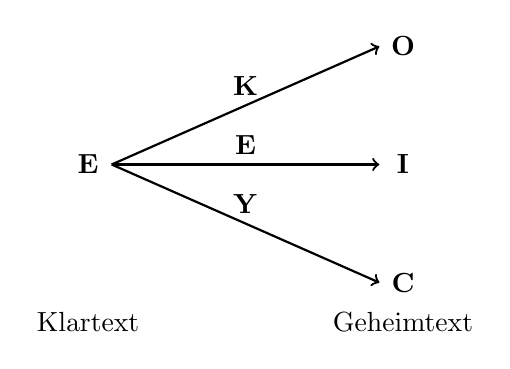
\begin{tikzpicture}
 % Klartext und Geheimtext Labels
 \node at (0, 0) {\textbf{E}};
 \node at (4, 1.5) {\textbf{O}};
 \node at (4, 0) {\textbf{I}};
 \node at (4, -1.5) {\textbf{C}};

 % Verbindungspfeile mit Schlüsseln
 \draw[->, thick] (0.3, 0) -- (3.7, 1.5) node[midway, above] {\textbf{K}};
 \draw[->, thick] (0.3, 0) -- (3.7, 0) node[midway, above] {\textbf{E}};
 \draw[->, thick] (0.3, 0) -- (3.7, -1.5) node[midway, above] {\textbf{Y}};

 % Labels Klartext und Geheimtext
 \node[align=center] at (0, -2) {Klartext};
 \node[align=center] at (4, -2) {Geheimtext};
\end{tikzpicture}
}

\newcommand{\vigenereFigTo}{
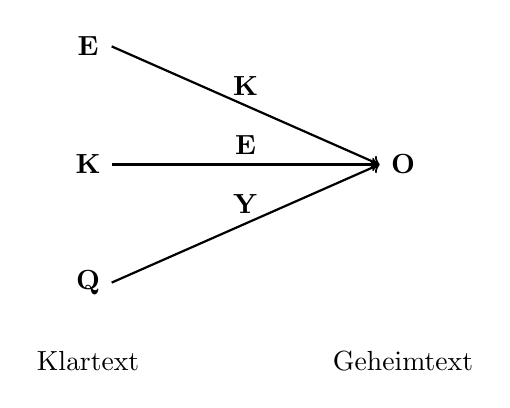
\begin{tikzpicture}
 % Klartext letters
 \node at (0, 1.5) {\textbf{E}};
 \node at (0, 0) {\textbf{K}};
 \node at (0, -1.5) {\textbf{Q}};
 
 % Geheimtext letter
 \node at (4, 0) {\textbf{O}};
 
 % Verbindungspfeile mit Schlüsseln
 \draw[->, thick] (0.3, 1.5) -- (3.7, 0) node[midway, above] {\textbf{K}};
 \draw[->, thick] (0.3, 0) -- (3.7, 0) node[midway, above] {\textbf{E}};
 \draw[->, thick] (0.3, -1.5) -- (3.7, 0) node[midway, above] {\textbf{Y}};
 
 % Labels Klartext und Geheimtext
 \node[align=center] at (0, -2.5) {Klartext};
 \node[align=center] at (4, -2.5) {Geheimtext};
\end{tikzpicture}
}

\newcommand{\vigenereFig}{
\begin{figure}[H]
	\centering
	\begin{subfigure}{.35\textwidth}
	\centering
	\resizebox{\textwidth}{!}{
	\vigenereFigFrom
	}
	\end{subfigure}
	\begin{subfigure}{.35\textwidth}
	\centering
	\resizebox{\textwidth}{!}{
	\vigenereFigTo}
	\end{subfigure}
	\end{figure}
	}
	
% Caesar dial, cleartext inside, cryptotext outside
\newcommand\caesar[1][3]{%
  \begin{tikzpicture}
    \def\r{2}
    \def\dr{0.5}
    \def\ri{1.4}
    \def\dri{0.5}
    \def\rotate{#1}%% number of shifts
    \coordinate (origin) at (0,0);
    \draw[fill=gray!60] (origin) circle (1pt);
    \draw (origin) circle (\r);
    \draw (origin) circle (\r+\dr);
    \draw (origin) circle (\ri);
    \draw (origin) circle (\ri+\dri);
    \foreach \letter [count=\ind from 0,evaluate=\ind as \ang using 90-\ind*360/26] in {A,B,...,Z}{%
        \node[rotate={\ang-90}] at ($(origin)+(\ang:{\r+\dr/2})$) {\textcolor{RoyalBlue}{\letter}};
        \draw({\ang+0.5*360/26}:\r)--({\ang+0.5*360/26}:\r+\dr);
      }
    \foreach \letter [count=\ind from 0,evaluate=\ind as \ang using 90-\ind*360/26-\rotate*360/26] in {A,B,...,Z}{%
        \node[rotate={\ang-90}] at ($(origin)+(\ang:{\ri+\dri/2})$) {\textcolor{ForestGreen}{\letter}};
        \draw({\ang+0.5*360/26}:\ri)--({\ang+0.5*360/26}:\ri+\dri);
      }
      \ifnumequal{\rotate}{0}{}{
      \draw[-latex] (90:\ri-0.3) arc (90:{90-\rotate*360/26}:\ri-0.3)node[pos=0.5,anchor=90-\rotate*180/26]{$\rotate$};}
    
  \end{tikzpicture}
}

% Caesar dial, cleartext outside, cryptotext inside
\newcommand\caesarreverse[1][3]{%
  \begin{tikzpicture}
    \def\r{2}
    \def\dr{0.5}
    \def\ri{1.4}
    \def\dri{0.5}
    \def\rotate{#1}%% number of shifts
    \coordinate (origin) at (0,0);
    \draw[fill=gray!60] (origin) circle (1pt);
    \draw (origin) circle (\r);
    \draw (origin) circle (\r+\dr);
    \draw (origin) circle (\ri);
    \draw (origin) circle (\ri+\dri);
    % Klartext AUSSEN (grün)
    \foreach \letter [count=\ind from 0, evaluate=\ind as \ang using 90-\ind*360/26-\rotate*360/26] in {A,B,...,Z}{%
        \node[rotate={\ang-90}] at ($(origin)+(\ang:{\r+\dr/2})$) {\textcolor{ForestGreen}{\letter}};
        \draw({\ang+0.5*360/26}:\r)--({\ang+0.5*360/26}:\r+\dr);
      }
    % Geheimtext INNEN (blau)
    \foreach \letter [count=\ind from 0, evaluate=\ind as \ang using 90-\ind*360/26] in {A,B,...,Z}{%
        \node[rotate={\ang-90}] at ($(origin)+(\ang:{\ri+\dri/2})$) {\textcolor{RoyalBlue}{\letter}};
        \draw({\ang+0.5*360/26}:\ri)--({\ang+0.5*360/26}:\ri+\dri);
      }
    % Pfeil AUSSEN mit Text OBEN
    \ifnumequal{\rotate}{0}{}{
      \draw[-latex] 
        (90:\r+\dr+0.3) 
        arc[start angle=90, end angle={90-\rotate*360/26}, radius=\r+\dr+0.3]
        node[midway, yshift=8pt] {$\rotate$};
    }
    
  \end{tikzpicture}
}


% code to generate a figure illustrating monoalphabetic substitution for a given substitution alphabet (first argument)
\newcommand{\multiKey}[1]{
\resizebox{\textwidth}{!}{
\begin{tikzpicture}[node distance=0.5cm and 0.5cm]
	\node(topL) at (-1,1.5) {};
	\node(bottomL) at (-1,0) {};
    % Erste Reihe (oberes Alphabet) automatisch generiert
    \foreach \i [count=\j from 1] in {A,...,Z} {
        \node (top\j) at (\j, 1.5) {\i};
    }

    % Zweite Reihe (unteres Alphabet) basierend auf dem Argument
    \foreach \i [count=\j from 1] in {#1} {
        \node (bottom\j) at (\j, 0) {\i};
    }

    % Verbindungen
    \foreach \i in {1,...,26} {
        \draw[<->] (top\i) -- (bottom\i);
    }
    
    % Zweiter Pfeil von bottomL nach topL, um 0.1cm nach rechts verschoben
    \draw[->,red,ultra thick] ($(bottomL.north)+(.5cm,0)$) -- node[right]{\emoji{key}}($(topL.south)+(.5cm,0)$);
    
    \draw[->,red,ultra thick] (topL) -- node[left]{\emoji{lock}} (bottomL);

\end{tikzpicture}
}
}